% !TEX root = ./cvl.tex
\section{Algorithms}
\label{sec:algorithms}

\subsection{Algorithmic framework}

The algorithmic framework is illustrated in Figure~\ref{fig:algorithmic-framework}

\begin{figure}[htbp]
\begin{center}
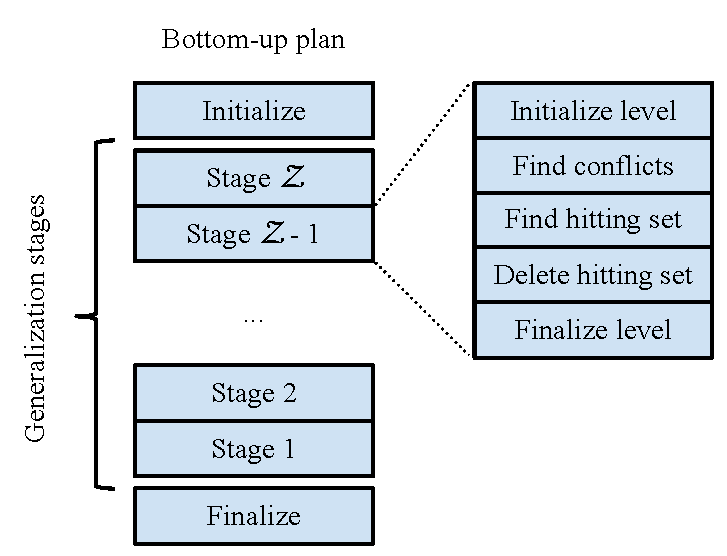
\includegraphics[scale=.7]{figs/cvl_stages.pdf}
\caption{The algorithmic framework}
\label{fig:algorithmic-framework}
\end{center}
\end{figure}


\subsection{Greedy algorithm}
Sorting based. Optimal for point datasets together with visibility constraint. @Martin: Recall that this algorithm is optimal when the subsets are disjoint (I have not proved this). 

\subsection{LP-rounding}

Described in Vazirani 14.1. @Martin: Please write here.

\subsection{Dual Fitting}

Described in Vazirani 13.2.1. @Martin: Please write here.


